Pada bab ini akan dijelaskan secara umum mengenai urutan pelaksanaan tugas akhir dengan langkah-langkah yang dilakukan.

\section{Studi Literatur}

Pada tahap ini dilakukan identifikasi permasalahan dan mengumpulkan informasi untuk memberi acuan pemecahan permasalahan. Studi literatur digunakan untuk mempelajari dan mengkaji lebih luas mengenai identitas-identitas yang akan digunakan dalam membantu menyelesaikan tugas akhir.

\subsection{Studi Lean}

Berdasarkan saran dari Prof. Kevin Buzzard, diperlukan waktu selama 11 minggu untuk studi pengoperasian Lean dengan tingkat kesulitan yang dibutuhkan untuk formalisasi \icm{}. Oleh karena itu, akan dilakukan terlebih dahulu pembelajaran formalisasi matematika menggunakan Lean di 11 minggu awal.

\subsection{Studi Aljabar Clifford}

Dilakukan studi intensif tentang aljabar Clifford bersamaan dengan studi Lean pada 11 minggu awal.

\section{Pembuktian Isomorfisma antara Aljabar Matriks dan Aljabar Clifford}

Setelah penulis memahami aljabar Clifford, dimulailah proses pembuktian \icm{}. Diberikan waktu selama 3 minggu untuk melakukan pembuktian ini.

\section{Formalisasi Isomorfisma antara Aljabar Matriks dan Aljabar Clifford}

\subsection{Formalisasi Sifat-sifat dasar Aljabar Clifford}

Sebagai langkah awal untuk uji coba awal dilakukan formalisasi sifat-sifat dasar aljabar Clifford yang telah dipelajari pada saat studi literatur.

\subsection{Formalisasi Isomorfisma untuk Dimensi Rendah}

Setelah berhasil dilakukan formalisasi sifat-sifat dasar, dimulai proses formalisasi \icm{} untuk dimensi-dimensi rendah terlebih dahulu, yaitu untuk isomorfisma yang sudah jelas seperti pada bilangan riil ${\operatorname{Cl}_{0,0} &\cong \mathbb{R}}$, bilangan kompleks ${\operatorname{Cl}_{0,1} &\cong \mathbb{C}}$, dan kuaternion ${\operatorname{Cl}_{0,2} &\cong \mathbb{H}}$.

\subsection{Formalisasi $\operatorname{Cl}_{p+1,q+1}(\mathbf{R}) = \mathrm{M}_2(\operatorname{Cl}_{p,q}(\mathbf{R}))$}

Akhirnya, formalisasi \icm{} menggunakan Lean. Diperhitungkan waktu selama 2 minggu cukup untuk mendapatkan formalisasi hasil tersebut.

\section{Penulisan Tugas Akhir}

Setelah semua tahapan penelitian selesai, disusun laporan tugas akhir mengenai penelitian yang telah dilakukan.

\section{Diagram Alir}

Adapun diagram alir proses tugas akhir ini diilustrasikan oleh Gambar 3.1.

\begin{figure}[H]
	\centering
	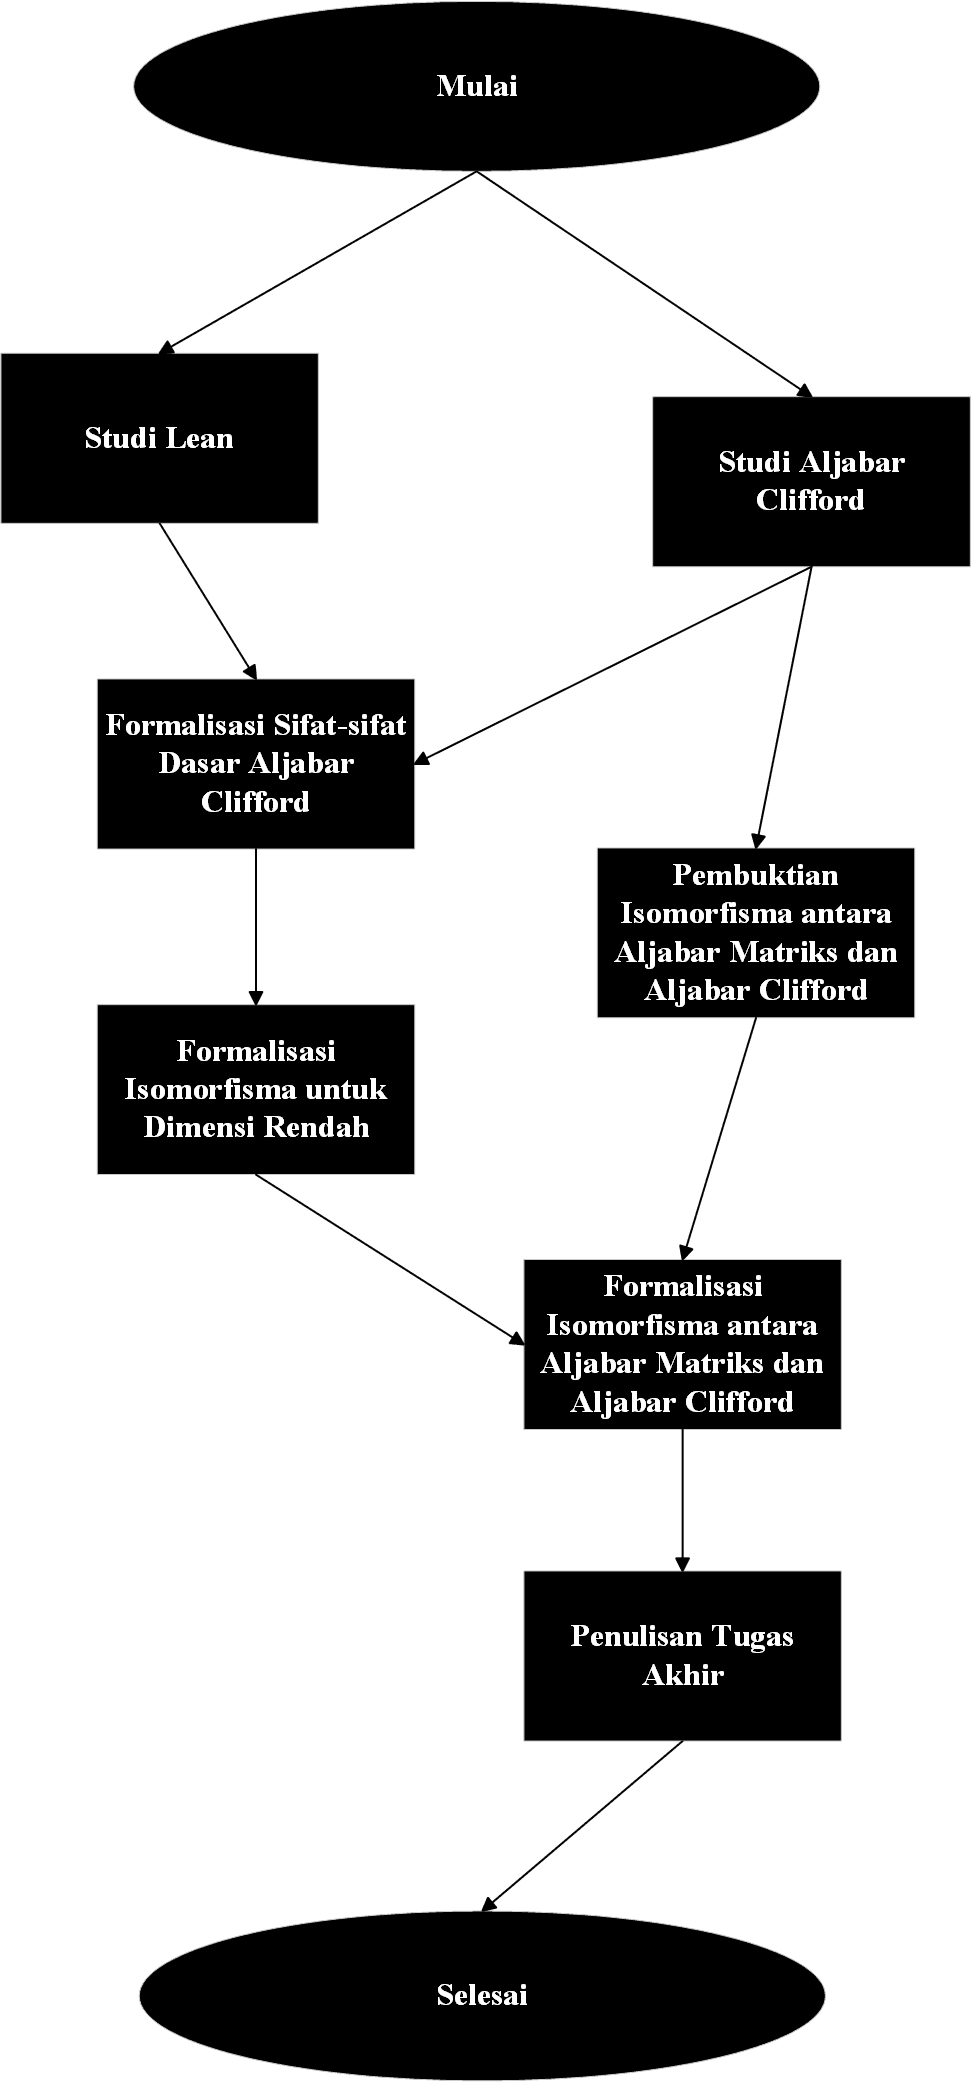
\includegraphics[width=8cm]{foto/BlockDiagram.png}
	\caption{Diagram Alir Metodologi.}
	\label{diagramalir}
\end{figure}

\section{Jadwal Kegiatan}
Berikut ini disajikan tabel jadwal kegiatan yang akan dilakukan selama 16 minggu dan berkoresponden dengan metodologi.\vspace{0.5cm}
% 	Membuat tabel

% Please add the following required packages to your document preamble:
% \usepackage{multirow}
% \usepackage[table,xcdraw]{xcolor}
% Beamer presentation requires \usepackage{colortbl} instead of \usepackage[table,xcdraw]{xcolor}
\begin{table}[H]
\caption{Jadwal Kegiatan}
\centering
\begin{tabular}{|c|l|lllllll|}
\hline
 & \multicolumn{1}{c|}{} & \multicolumn{7}{c|}{\textbf{Minggu}} \\ \cline{3-9}
\multirow{-2}{*}{\textbf{No}} & \multicolumn{1}{c|}{\multirow{-2}{*}{\textbf{Nama Kegiatan}}} & \multicolumn{1}{l|}{1 sampai 10} & \multicolumn{1}{l|}{11} & \multicolumn{1}{l|}{12} & \multicolumn{1}{l|}{13} & \multicolumn{1}{l|}{14} & \multicolumn{1}{l|}{15} & 16 \\ \hline
1 & Studi Lean & \multicolumn{1}{l|}{\cellcolor[HTML]{000000}} & \multicolumn{1}{l|}{\cellcolor[HTML]{000000}} & \multicolumn{1}{l|}{} & \multicolumn{1}{l|}{} & \multicolumn{1}{l|}{} & \multicolumn{1}{l|}{} &  \\ \hline
2 & Studi Aljabar Clifford & \multicolumn{1}{l|}{\cellcolor[HTML]{000000}{\color[HTML]{000000} }} & \multicolumn{1}{l|}{\cellcolor[HTML]{000000}} & \multicolumn{1}{l|}{} & \multicolumn{1}{l|}{} & \multicolumn{1}{l|}{} & \multicolumn{1}{l|}{} &  \\ \hline
3 & \begin{tabular}[c]{@{}l@{}}Pembuktian Isomorfisma antara\\ Aljabar Matriks dan Aljabar Clifford\end{tabular} & \multicolumn{1}{l|}{} & \multicolumn{1}{l|}{} & \multicolumn{1}{l|}{\cellcolor[HTML]{000000}{\color[HTML]{000000} }} & \multicolumn{1}{l|}{\cellcolor[HTML]{000000}{\color[HTML]{000000} }} & \multicolumn{1}{l|}{\cellcolor[HTML]{000000}{\color[HTML]{000000} }} & \multicolumn{1}{l|}{} &  \\ \hline
4 & \begin{tabular}[c]{@{}l@{}}Formalisasi Sifat-sifat Dasar\\ Aljabar Clifford\end{tabular} & \multicolumn{1}{l|}{} & \multicolumn{1}{l|}{\cellcolor[HTML]{000000}} & \multicolumn{1}{l|}{} & \multicolumn{1}{l|}{} & \multicolumn{1}{l|}{} & \multicolumn{1}{l|}{} &  \\ \hline
5 & \begin{tabular}[c]{@{}l@{}}Formalisasi Isomorfisma untuk\\ Dimensi Rendah\end{tabular} & \multicolumn{1}{l|}{} & \multicolumn{1}{l|}{} & \multicolumn{1}{l|}{\cellcolor[HTML]{000000}} & \multicolumn{1}{l|}{} & \multicolumn{1}{l|}{} & \multicolumn{1}{l|}{} &  \\ \hline
6 & \begin{tabular}[c]{@{}l@{}}Formalisasi Isomorfisma antara\\ Aljabar Matriks dan Aljabar Clifford\end{tabular} & \multicolumn{1}{l|}{} & \multicolumn{1}{l|}{} & \multicolumn{1}{l|}{} & \multicolumn{1}{l|}{\cellcolor[HTML]{000000}} & \multicolumn{1}{l|}{\cellcolor[HTML]{000000}} & \multicolumn{1}{l|}{} &  \\ \hline
7 & Penulisan Tugas Akhir & \multicolumn{1}{l|}{} & \multicolumn{1}{l|}{} & \multicolumn{1}{l|}{} & \multicolumn{1}{l|}{} & \multicolumn{1}{l|}{} & \multicolumn{1}{l|}{\cellcolor[HTML]{000000}{\color[HTML]{000000} }} & \cellcolor[HTML]{000000}{\color[HTML]{000000} } \\ \hline
\end{tabular}
\end{table}
